
%(BEGIN_QUESTION)
% Copyright 2007, Tony R. Kuphaldt, released under the Creative Commons Attribution License (v 1.0)
% This means you may do almost anything with this work of mine, so long as you give me proper credit

This pneumatic controller exhibits a characteristic equation called the {\it series} or {\it interacting} equation:

$$\includegraphics[width=15.5cm]{i04458x01.eps}$$

$$m = K_p \left[ \left({\tau_d \over \tau_i} + 1 \right) e + {1 \over \tau_i} \int e \> dt + \tau_d {de \over dt} \right]$$

\vskip 10pt

Identify which valves influence the aggressiveness of the P, I, and D control actions in this mechanism.  

\vskip 10pt

\begin{itemize}
\item{} Valve(s) influencing the controller's proportional action:
\vskip 10pt
\item{} Valve(s) influencing the controller's integral action:
\vskip 10pt
\item{} Valve(s) influencing the controller's derivative action:
\vskip 10pt
\item{} Which direction to move the fulcrum for a {\it greater} proportional band: ({\it left} or {\it right})
\end{itemize}

\underbar{file i04458}
%(END_QUESTION)





%(BEGIN_ANSWER)

I recommend 4 points for the proportional action answer, plus 2 points for each other answer:

\vskip 10pt

Valve(s) influencing the controller's proportional action: ${\bf V_1}$ and ${\bf V_2}$

\vskip 10pt

Valve(s) influencing the controller's integral action: ${\bf V_1}$ 

\vskip 10pt

Valve(s) influencing the controller's derivative action: ${\bf V_2}$ 

\vskip 10pt

Which direction to move the fulcrum for a {\it greater} proportional band: {\bf right}


%(END_ANSWER)





%(BEGIN_NOTES)

{\bf This question is intended for exams only and not worksheets!}.

%(END_NOTES)


